% !TeX root = proyecto.tex
%=========================================================
\chapter{Modelo de la interacción}	
\label{cap:modInteraccion}

\cdtInstrucciones{Introduzca el capítulo indicando su contenido y organización.}	

\cdtInstrucciones{Utilice este capítulo para describir todos los detalles de la interacción con el usuario, describiendo elementos d eusabilidad, ergonomía, psicología,  arqjuitectura de información y repreentación.}

Este capítulo describe ...
\clearpage
\section{Modelo de navegación}

\cdtInstrucciones{Describa de acuerdo al tipo de aplicación como es la interacción con el usuario, destacando los elementos de ubicación dentro de la aplicación. Si las interfaces tiene elementos comunes más allá de los que son comunes a todas las aplicaciones describalos ampliamente así como los encabezados, pies de página, menús y otros elementos que aparecen repetitivamente entre las pantallas.}

	La navegación entre pantallas se muestra en la figura~\ref{fig:mapa}. en el se explica ...\\

\begin{figure}[h]
	\begin{center}
		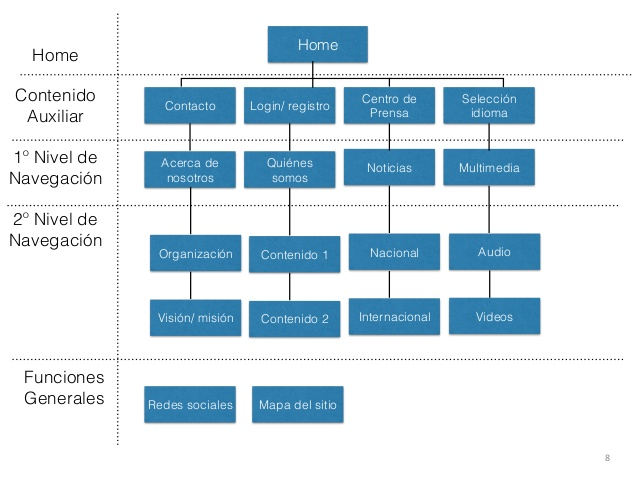
\includegraphics[width=.5\textwidth]{images/mapa}
		\caption{mapa}
		\label{fig:mapa}
	\end{center}
\end{figure}


\cdtInstrucciones{A continuación describa cada una de las pantallas.}
%% !TeX root = ../proyecto.tex
%--------------------------------------
\section{IUX Interfaz (nombre de la interfaz)}

\subsection{Objetivo}
	\cdtInstrucciones{Describa el objetivo, propósito o función de la pantalla.}

\subsection{Diseño}
	\cdtInstrucciones{Describa brevemente los elementos de la pantalla y como de be usarse a manera de manual de usuario.} Esta pantalla \IUref{IU23}{Pantalla de Control de Acceso} aparece al iniciar el sistema, para ingresar ... 

\IUfig[.7]{Login}{IU23}{Pantalla de Control de Acceso.}

%\IUfig[ancho de la figura: valor entre 1 y .1]{Nombre corto de la pantalla sin espacions ni acentos}{IUXX}{Nombre largo de la pantalla.}

\subsection{Salidas}

	\cdtInstrucciones{Liste las salidas de la interfaz. Si coinciden con las del caso de uso solo indiquelo. Esta ,ista debe incluir los mensajes}

	\begin{itemize}
		\item Descripción de salida.
	\end{itemize}
	
\subsection{Entradas}

	\cdtInstrucciones{Liste las entradas de la interfaz. Si coinciden con las del caso de uso solo indiquelo.}
	\begin{itemize}
		\item Descripción de salida.
	\end{itemize}

\subsection{Comandos}
	\cdtInstrucciones{Describa cada control (botónes, areas de drag and drop, componentes interactivos, animaciones, etc.) que se puede utilizar dentro de la pantalla indicando o que hacen y si cambia de pantalla.}

\begin{itemize}
	\item \IUbutton{Entrar}: Verifica que el Estudiante se encuentre registrado y la contraseña sea la correcta. Si la verificación es correcta, se muestra la \IUref{UI32}{Pantalla de Selección de Seminario}.
	\item \IUbutton{Ayuda}: Muestra la ayuda de esta pantalla \IUref{IU50}{Pantalla de Ayuda}.
\end{itemize}


% !TeX root = ../proyecto.tex
%--------------------------------------
\section{IU001 Interfaz (Control de acceso)}

\subsection{Objetivo}
	\cdtInstrucciones{Describa el objetivo, propósito o función de la pantalla.}
Esta Interfaz tiene como objetivo permitir al usuario introducir sus datos para acceder al sistema.
\subsection{Diseño}
	\cdtInstrucciones{Describa brevemente los elementos de la pantalla y como de be usarse a manera de manual de usuario.} 
 Esta pantalla \IUref{IU001}{Pantalla de Control de Acceso} aparece al iniciar el sistema, para ingresar su identificador tiene un cmpo de texto en la parte de arriba, un campo de contraseña para ingresar su contraseña, debajo un boton para enviar el formulario y finalmente un hipervinculo para acceder a la recuperacion de contraseña. 

\IUfig[.7]{IU001}{IU001}{Pantalla de Control de Acceso.}

%\IUfig[ancho de la figura: valor entre 1 y .1]{Nombre corto de la pantalla sin espacions ni acentos}{IUXX}{Nombre largo de la pantalla.}

\subsection{Salidas}

	\cdtInstrucciones{Liste las salidas de la interfaz. Si coinciden con las del caso de uso solo indiquelo. Esta ,ista debe incluir los mensajes}

	\begin{itemize}
		\item Coincide con el caso de uso
	\end{itemize}
	
\subsection{Entradas}

	\cdtInstrucciones{Liste las entradas de la interfaz. Si coinciden con las del caso de uso solo indiquelo.}
	\begin{itemize}
		\item Coincide con el caso de uso.
	\end{itemize}

\subsection{Comandos}
	\cdtInstrucciones{Describa cada control (botónes, areas de drag and drop, componentes interactivos, animaciones, etc.) que se puede utilizar dentro de la pantalla indicando o que hacen y si cambia de pantalla.}

\begin{itemize}
	\item \IUbutton{Entrar}: Verifica los datos del formulario esten llenos, el id exista, la contraseña coincida con la guardada y la cuenta no este suspendida, ademas busca el rol del perfil. Si la verificación es correcta, se muestra la \IUref{IU-003}{Pantalla Principal}.
	\item \IUbutton{Recuperr Contraseña}:Se muestra la \IUref{IU-004}{Recuperar contraseña}.
\end{itemize}


% !TeX root = ../proyecto.tex
%--------------------------------------
\section{IU003 Interfaz (Pagina Principal)}

\subsection{Objetivo}
	\cdtInstrucciones{Describa el objetivo, propósito o función de la pantalla.}
Esta Interfaz tiene como objetivo permitir al usuario una facil navegación a traves del sistema y las funcionalidades que el puede usar.
\subsection{Diseño}
	\cdtInstrucciones{Describa brevemente los elementos de la pantalla y como de be usarse a manera de manual de usuario.} Esta pantalla \IUref{IU003}{Pantalla Principal} aparece al acceder al sistema, consta de un menu desplegable con las siguientes categorias, nombre, materias,escuela .

\IUfig[.7]{IU003}{IU003}{Pantalla Principal.}

%\IUfig[ancho de la figura: valor entre 1 y .1]{Nombre corto de la pantalla sin espacions ni acentos}{IUXX}{Nombre largo de la pantalla.}

\subsection{Salidas}

	\cdtInstrucciones{Liste las salidas de la interfaz. Si coinciden con las del caso de uso solo indiquelo. Esta ,ista debe incluir los mensajes}

	\begin{itemize}
		\item Notificaciones
	\end{itemize}
	
\subsection{Entradas}

	\cdtInstrucciones{Liste las entradas de la interfaz. Si coinciden con las del caso de uso solo indiquelo.}
	\begin{itemize}
		\item Ninguna.
	\end{itemize}

\subsection{Comandos}
	\cdtInstrucciones{Describa cada control (botónes, areas de drag and drop, componentes interactivos, animaciones, etc.) que se puede utilizar dentro de la pantalla indicando o que hacen y si cambia de pantalla.}

\begin{itemize}
	\item \IUbutton{Entrar}: Verifica los datos del formulario esten llenos, el id exista, la contraseña coincida con la guardada y la cuenta no este suspendida, ademas busca el rol del perfil. Si la verificación es correcta, se muestra la \IUref{IU-003}{Pantalla Principal}.
	\item \IUbutton{Recuperr Contraseña}:Se muestra la \IUref{IU-004}{Recuperar contraseña}.
\end{itemize}


% !TeX root = ../proyecto.tex
%--------------------------------------
\section{IU004 Interfaz (Recuperar contraseña)}

\subsection{Objetivo}
	\cdtInstrucciones{Describa el objetivo, propósito o función de la pantalla.}
Esta Interfaz tiene como objetivo permitir al usuario recuperar su contraseña si la olvido pero recuerda su identificador y su correo.
\subsection{Diseño}
	\cdtInstrucciones{Describa brevemente los elementos de la pantalla y como de be usarse a manera de manual de usuario.} Esta pantalla \IUref{IU004}{Recuperar contraseña} contiene solo dos campos de texto y un botón para enviar el formulario .

\IUfig[.7]{IU004}{IU004}{Recuperar contraseña.}

%\IUfig[ancho de la figura: valor entre 1 y .1]{Nombre corto de la pantalla sin espacions ni acentos}{IUXX}{Nombre largo de la pantalla.}

\subsection{Salidas}

	\cdtInstrucciones{Liste las salidas de la interfaz. Si coinciden con las del caso de uso solo indiquelo. Esta ,ista debe incluir los mensajes}

	\begin{itemize}
		\item Igual al caso de uso
	\end{itemize}
	
\subsection{Entradas}

	\cdtInstrucciones{Liste las entradas de la interfaz. Si coinciden con las del caso de uso solo indiquelo.}
	\begin{itemize}
		\item Igual al caso de uso.
	\end{itemize}

\subsection{Comandos}
	\cdtInstrucciones{Describa cada control (botónes, areas de drag and drop, componentes interactivos, animaciones, etc.) que se puede utilizar dentro de la pantalla indicando o que hacen y si cambia de pantalla.}

\begin{itemize}
	\item \IUbutton{Recuperar}: Verifica los datos del formulario esten llenos, el id exista, la cuenta no este suspendida, y que el correo coincida con el guarddo. Si la verificación es correcta, se muestra la \IUref{IU-001}{Control de acceso}.
	
\end{itemize}


% !TeX root = ../proyecto.tex
%--------------------------------------
\section{IU005 Interfaz (Registro Centro de Trabajo)}

\subsection{Objetivo}
	\cdtInstrucciones{Describa el objetivo, propósito o función de la pantalla.}
 Esta Interfaz tiene como objetivo permitir al usuario introducir nuevos centros de trabajo, claves de centro de trabajo y/o prestamos de las mismas al programa.

\subsection{Diseño}
	\cdtInstrucciones{Describa brevemente los elementos de la pantalla y como de be usarse a manera de manual de usuario.} Esta pantalla \IUref{IU005}{Registro Centro de Trabajo} aparece al seleccionar la opción en el menú, contiene 5 campos de texto que deben ser llenados con los datos del Centro de trabajo, tambien tiene 2 seletores y un boton para intentar guardar los datos.
\clearpage
\IUfig[.5]{IU005}{IU005}{Registro Centro de Trabajo.}

%\IUfig[ancho de la figura: valor entre 1 y .1]{Nombre corto de la pantalla sin espacions ni acentos}{IUXX}{Nombre largo de la pantalla.}

\subsection{Salidas}

	\cdtInstrucciones{Liste las salidas de la interfaz. Si coinciden con las del caso de uso solo indiquelo. Esta ,ista debe incluir los mensajes}

	\begin{itemize}
		\item Coincide con el caso.
	\end{itemize}
	
\subsection{Entradas}

	\cdtInstrucciones{Liste las entradas de la interfaz. Si coinciden con las del caso de uso solo indiquelo.}
	\begin{itemize}
		\item Coincide con el caso.
	\end{itemize}

\subsection{Comandos}
	\cdtInstrucciones{Describa cada control (botónes, areas de drag and drop, componentes interactivos, animaciones, etc.) que se puede utilizar dentro de la pantalla indicando o que hacen y si cambia de pantalla.}

\begin{itemize}
	\item \IUbutton{Registrar}: Verifica que los datos introducidos sean validos y tengan el formato correcto, de ser asi guardara el nuevo centro de trabajo limpiando el formulario.
	
\end{itemize}


% !TeX root = ../proyecto.tex
%--------------------------------------
\section{IU006 Interfaz (registro de Salon)}

\subsection{Objetivo}
	\cdtInstrucciones{Describa el objetivo, propósito o función de la pantalla.}

\subsection{Diseño}
	\cdtInstrucciones{Describa brevemente los elementos de la pantalla y como de be usarse a manera de manual de usuario.} Esta pantalla \IUref{IU001}{Pantalla de Control de Acceso} aparece al iniciar el sistema, para ingresar ... 

\IUfig[.5]{IU006}{IU006}{Registro de salon.}

%\IUfig[ancho de la figura: valor entre 1 y .1]{Nombre corto de la pantalla sin espacions ni acentos}{IUXX}{Nombre largo de la pantalla.}

\subsection{Salidas}

	\cdtInstrucciones{Liste las salidas de la interfaz. Si coinciden con las del caso de uso solo indiquelo. Esta ,ista debe incluir los mensajes}

	\begin{itemize}
		\item Descripción de salida.
	\end{itemize}
	
\subsection{Entradas}

	\cdtInstrucciones{Liste las entradas de la interfaz. Si coinciden con las del caso de uso solo indiquelo.}
	\begin{itemize}
		\item Descripción de salida.
	\end{itemize}

\subsection{Comandos}
	\cdtInstrucciones{Describa cada control (botónes, areas de drag and drop, componentes interactivos, animaciones, etc.) que se puede utilizar dentro de la pantalla indicando o que hacen y si cambia de pantalla.}

\begin{itemize}
	\item \IUbutton{Entrar}: Verifica que el Estudiante se encuentre registrado y la contraseña sea la correcta. Si la verificación es correcta, se muestra la \IUref{UI32}{Pantalla de Selección de Seminario}.
	\item \IUbutton{Ayuda}: Muestra la ayuda de esta pantalla \IUref{IU50}{Pantalla de Ayuda}.
\end{itemize}


% !TeX root = ../proyecto.tex
%--------------------------------------
\section{IU007 Interfaz (Asignación de Director)}

\subsection{Objetivo}
	\cdtInstrucciones{Describa el objetivo, propósito o función de la pantalla.}

\subsection{Diseño}
	\cdtInstrucciones{Describa brevemente los elementos de la pantalla y como de be usarse a manera de manual de usuario.} Esta pantalla \IUref{IU007}{Asignación de Director} aparece al iniciar el sistema, para ingresar ... 

\IUfig[.7]{IU007}{IU007}{Asignación de Director.}

%\IUfig[ancho de la figura: valor entre 1 y .1]{Nombre corto de la pantalla sin espacions ni acentos}{IUXX}{Nombre largo de la pantalla.}

\subsection{Salidas}

	\cdtInstrucciones{Liste las salidas de la interfaz. Si coinciden con las del caso de uso solo indiquelo. Esta ,ista debe incluir los mensajes}

	\begin{itemize}
		\item Descripción de salida.
	\end{itemize}
	
\subsection{Entradas}

	\cdtInstrucciones{Liste las entradas de la interfaz. Si coinciden con las del caso de uso solo indiquelo.}
	\begin{itemize}
		\item Descripción de salida.
	\end{itemize}

\subsection{Comandos}
	\cdtInstrucciones{Describa cada control (botónes, areas de drag and drop, componentes interactivos, animaciones, etc.) que se puede utilizar dentro de la pantalla indicando o que hacen y si cambia de pantalla.}

\begin{itemize}
	\item \IUbutton{Entrar}: Verifica que el Estudiante se encuentre registrado y la contraseña sea la correcta. Si la verificación es correcta, se muestra la \IUref{UI32}{Pantalla de Selección de Seminario}.
	\item \IUbutton{Ayuda}: Muestra la ayuda de esta pantalla \IUref{IU50}{Pantalla de Ayuda}.
\end{itemize}


%!TEX root = ejemplo.tex
%=========================================================
\section{Catálogo de mensajes}	
\label{sec:mensajes}

	En esta sección se describen todos los mensajes que aparecen en el sistema. Para cada mensaje se especifica:
	 
	\begin{description}\itemsep0em
		\item[Id:] Identificador del mensaje de la forma ``MSG XX'' y descripción corta del mismo.
		\item[Tipo:] Tipo del mensaje el cual puede ser: 
		\begin{description}
			\item[Normal:] Mensaje que informa al usuario una instrucción o el estado interno que guarda el sistema, suele tener un color {\color{msgNormalColor}Azul}.
			\item[Éxito:] Mensaje que informa al usuario sobre una acción realizada, sirve para confirmar el correcto funcionamiento del sistema. Se presentan con un color {\color{msgInfoColor}Verde}.
			\item[Atención:] Mensaje que tiene como finalidad llamar la atención del usuario a una situación que requiere su intervención, por ejemplo cuando una actividad ha generado un efecto colateral o se realizará una acción destructiva y no reversible. Se presentan con un color {\color{msgWarningColor}Naranja}.
			\item[Error:] Mensaje que informa al usuario un fallo en en una operación o un impedimento para realizarla, por ejemplo: cuando no se puede efectuar la acción solicitada, cuando un dato falta o tiene un formato no aceptado por el sistema. Se presentan con un color {\color{msgErrorColor}Rojo}.
		\end{description}
		\item[Propósito:] Explicación del propósito del mensaje.
		\item[Redacción:] Redacción del mensaje.
		\item[Parámetros:] En caso de que el mensaje pueda variar se especifican los casos y la forma en que debe adaptarse la redacción
		\item[Ejemplos:] Ejemplos de como debe renderizarse el mensaje.
	\end{description}


\subsection{Lista de mensajes}

%msgNormalColor
%msgInfoColor
%msgWarningColor
%msgErrorColor

%Mensajes de error relacionado al inicio de secion (Origen CU-001)

\begin{cdtMessage}[msgInfoColor]{MSG-001}{Bienvenida al usuario}
	\item[Propósito:] Indicar al usuario que ha ingresado satisfactoriamente al sistema.
	\item[Redacción:] Bienvenido $<$nombre$>$ $<$Primer Apellido$>$.
	\item[Parámetros:] \hspace{1cm}
	\begin{itemize}
		\item $<$nombre$>$ \hyperlink{Usuario.nombre}{Nombre} del Usuario.
  \item $<$Primer Apellido$>$ \hyperlink{Usuario.primerApellido}{Primer Apellido} del Usuario.
	\end{itemize}
	\item[Ejemplos:] Bienvenido Juan Pérez.
\end{cdtMessage}

\begin{cdtMessage}[msgErrorColor]{MSG-002}{Usuario no registrado} 
	\item[Propósito:] Indica que el usuario ingresado no existe en el sistema.
	\item[Redacción:] El usuario $<$Identificador$>$ no se encuentra registrado.
	\item[Parámetros:] \hspace{1cm}
	\begin{itemize}
		\item $<$Identificador$>$ \hyperlink{Usuario.ID}{Identificador} del Usuario.
	\end{itemize}
	\item[Ejemplos:] El usuario 123123 no se encuentra registrado.
\end{cdtMessage}

\begin{cdtMessage}[msgErrorColor]{MSG-003}{Cuenta inactiva} 
	\item[Propósito:] Indicar al usuario que la cuenta especificada se encuentra inactiva.
	\item[Redacción:] La cuenta especificada $<$ID$>$ se encuentra inactiva.
	\item[Parámetros:] \hspace{1cm}
	\begin{itemize}
		\item $<$ID$>$ \hyperlink{Usuario.ID}{Identificador} del Usuario.
	\end{itemize}
	\item[Ejemplos:] La cuenta especificada 123123 se encuentra inactiva.
\end{cdtMessage}

\begin{cdtMessage}[msgErrorColor]{MSG-004}{Error de inicio de sesión}
	\item[Propósito:] Indica al usuario que la contraseña introducida es incorrecta.
	\item[Redacción:] La contraseña ingresada es incorrecta.
	\item[Parámetros:] No aplica.
	\item[Ejemplos:] La contraseña ingresada es incorrecta.
\end{cdtMessage}

\begin{cdtMessage}[msgErrorColor]{MSG-005}{Faltan Campos Obligatorios} 
	\item[Propósito:] Indicar al usuario que olvido agregar algún campo obligtorio.
	\item[Redacción:] El campo $<$campo$>$ es obligatorio y se encuentra vacio.
	\item[Parámetros:] \hspace{1cm}
	\begin{itemize}
		\item $<$campo$>$ de la IU.
	\end{itemize}
	\item[Ejemplos:] El campo contraseña es obligatorio y se encuentra vacio.
\end{cdtMessage}

%Mensajes de informacion no compatible con los filtros (CU002)

\begin{cdtMessage}[msgInfoColor]{MSG-006}{No se encontró información} 
	\item[Propósito:] Indicar al usuario que no existen elementos que cumplan con los filtros establecidos.
	\item[Redacción:] Ningún elemento cumple con los filtros puestos.
	\item[Parámetros:] \hspace{1cm}
	\begin{itemize}
		\item No aplica.
	\end{itemize}
	\item[Ejemplos:] Se puso de filtro un nombre de escuela que no existe, ergo no muestra ningún elemento.
\end{cdtMessage}

%Mensajes de error relacionados con tiempo (Duda de que CU de origen)
\begin{cdtMessage}[msgErrorColor]{MSG-007}{Campo con formato incorrecto} 
	\item[Propósito:] Indicar al usuario que el contenido de uno de sus campos no cumple con el formato requerido.
	\item[Redacción:] El campo $<$campo$>$ no cumple con el formato especificado, favor de corroborarlo.
	\item[Parámetros:] \hspace{1cm}
	\begin{itemize}
		\item $<$campo$>$ de la IU.
	\end{itemize}
	\item[Ejemplos:] El campo CURP no cumple con el formato especificado, favor de corroborarlo.
\end{cdtMessage}
\begin{cdtMessage}{MSG-008}{Tiempo restante para terminar un proceso} 
	\item[Propósito:] Indicar al usuario el tiempo restante para terminar una operación limitada en el tiempo como la reinscripción.
	\item[Redacción:] Quedan $<$tiempo$>$ para terminar la $<$operación$>$.
	\item[Parámetros:] \hspace{1cm}
	\begin{itemize}
		\item $<$tiempo$>$ Tiempo faltante para la operació especificando días, horas minutos y segundos.
		\item 
	\end{itemize}
	\item[Ejemplos:] \hspace{1cm}
	\begin{itemize}
		\item Quedan 45 días, 2 horas 12 minutos y 45 segundos para iniciar tu reinscripción.
		\item Quedan 2 minutos y 32 segundos para terminar tu reinscripción
	\end{itemize}
\end{cdtMessage}

\begin{cdtMessage}[msgInfoColor]{MSG-009}{Operación exitosa}
	\item[Propósito:] Informar al usuario que la operación solicitada ha sido ejecutada con éxito.
	\item[Redacción:] $<$Artículo$>$ $<$Operación$>$ del $<$Entidad$>$ $<$Identificador$>$ se realizó con éxito.
	\item[Parámetros:]\hspace{1pt}
	\begin{itemize}
		\item $<$Artículo$>$ $<$Operación$>$ se refiere a la operación realizada.
		\item $<$Entidad$>$ $<$Identificador$>$ se refiere al elemento del negocio donde recayó la operación, indicando el tipo del objeto y un dato que el usuario pueda usar para identificarlo.
	\end{itemize}
	\item[Ejemplo:] Algunos ejemplos son
	\begin{itemize}
		\item El registro del Alumno 342343 se realizó con éxito.
		\item La eliminación de la Tarea ``documentar el proceso'' se ha realizado con éxito.
	\end{itemize}
\end{cdtMessage}
\begin{cdtMessage}[msgErrorColor]{MSG-010}{Clave del Centro de Trabajo no Prestada} 
	\item[Propósito:] Indicar al usuario que la clave de centro de trabajo proporcionada no permite ser prestado.
	\item[Redacción:] La CCT proporcionada no permite ser prestada, por favor ponerse en contacto con el director del Centro de Trabajo propietario.
	\item[Parámetros:] \hspace{1cm}
	\begin{itemize}
		\item No aplica.
	\end{itemize}
	\item[Ejemplos:] La CCT proporcionada no permite ser prestada, por favor ponerse en contacto con el director del Centro de Trabajo propietario.
\end{cdtMessage}
\begin{cdtMessage}[msgInfoColor]{MSG-011}{registro exitoso}
	\item[Propósito:] Indicar al usuario que ha registrado satisfactoriamente un nuevo registro.
	\item[Redacción:] Se ha completado el registro de $<$nombre$>$ .
	\item[Parámetros:] \hspace{1cm}
	\begin{itemize}
		\item $<$nombre$>$ \hyperlink{Usuario.nombre}{Nombre} del Usuario.
	\end{itemize}
	\item[Ejemplos:] Se ha completado el registro de un Centro de Trabajo
\end{cdtMessage}
\begin{cdtMessage}[msgErrorColor]{MSG-012}{Fecha anterior a la fecha actual} 
	\item[Propósito:] Indicar al usuario que la fecha seleccionada es anterior a la fecha actual.
	\item[Redacción:] La fecha proporcionada es anterior al día de hoy por lo que no se puede admitir.
	\item[Parámetros:] \hspace{1cm}
	\begin{itemize}
		\item No aplica
	\end{itemize}
	\item[Ejemplos:]  La fecha proporcionada es anterior al día de hoy por lo que no se puede admitir.
\end{cdtMessage}
